In this analysis, quarks or gluons can be produced via the strong interaction from a hard scattering process.
Due to QCD colr confinement, these strong interaction particles can emit soft gluons producing quark and anti-quark pairs or gluons, ending up with colorless particles, hadrons.
Some unstable hadrons then decay immediately to stable particles such as other hadrons, photons, or leptons, forming a shower of particles called jets.
It is common to cluster these showers as a single object to represent the underlying parton.

\subsection{Jet reconstruction}
Jets are reconstructed by clustering showers of the particle-flow candidates.
The clustering algorithm compares two different distance measures $d_i$ and $d_{ij}$ and update the jet candidates to complete the process.
The $d_i$ is the distance between the original beam and the particle $i$ from an existing list of particles.
The $d_{ij}$ is the distance between the particle $i$ and a half constructed pseudo-jet.
The two distance measures are given as
\begin{linenomath}\begin{equation}\begin{aligned}\label{eq:reco_anti_kt}
    d_{i}  &= p_{\mathrm{T},i}^{2p}  \\
    d_{ij} &= min[p_{\mathrm{T},i}^{2p}, p_{\mathrm{T},j}^{2p}] \times \frac{\Delta^2_{ij}}{R^2}
\end{aligned}\end{equation}\end{linenomath}
where $p_{\mathrm{T},i}$ is the transverse momentum of particle $i$, $p_{\mathrm{T},j}$ is the transverse momentum of the pseudo-jet, $\Delta_{ij}$ is the angular separation of the particle $i$ and pseudo-jet $j$, $R$ is some angular size parameter defined by user, and $p$ is also a factor that is defined by the user.
The particle $i$ with $d_{ij}$ smaller than $d_i$ is considered close to the pseudo-jet $j$ and thus is merged into the pseudo-jet object.
The kinematics of the pseudo-jet object are then re-computed, and the particle $i$ is removed from the original particle list.
This process is complete when no particle can be added to the pseudo-jet, and a new pseudo-jet is created with the largest \PT particle in the remaining particle list.

This clustering algorithm is commonly used in the CMS experiment with the value of $p=-1$, and thus referred to the anti-\kt algorithm~\cite{CMS:antikt}.
This algorithm allows the jet clustering to be less sensitive to the existence of particles originating from soft processes and thus making itself less sensitive to the high pileup situation, as shown in Fig.~\ref{fig:reco_antikt.png}.
The size parameter used in this analysis is $R=0.4$.
\begin{figure}\centering
    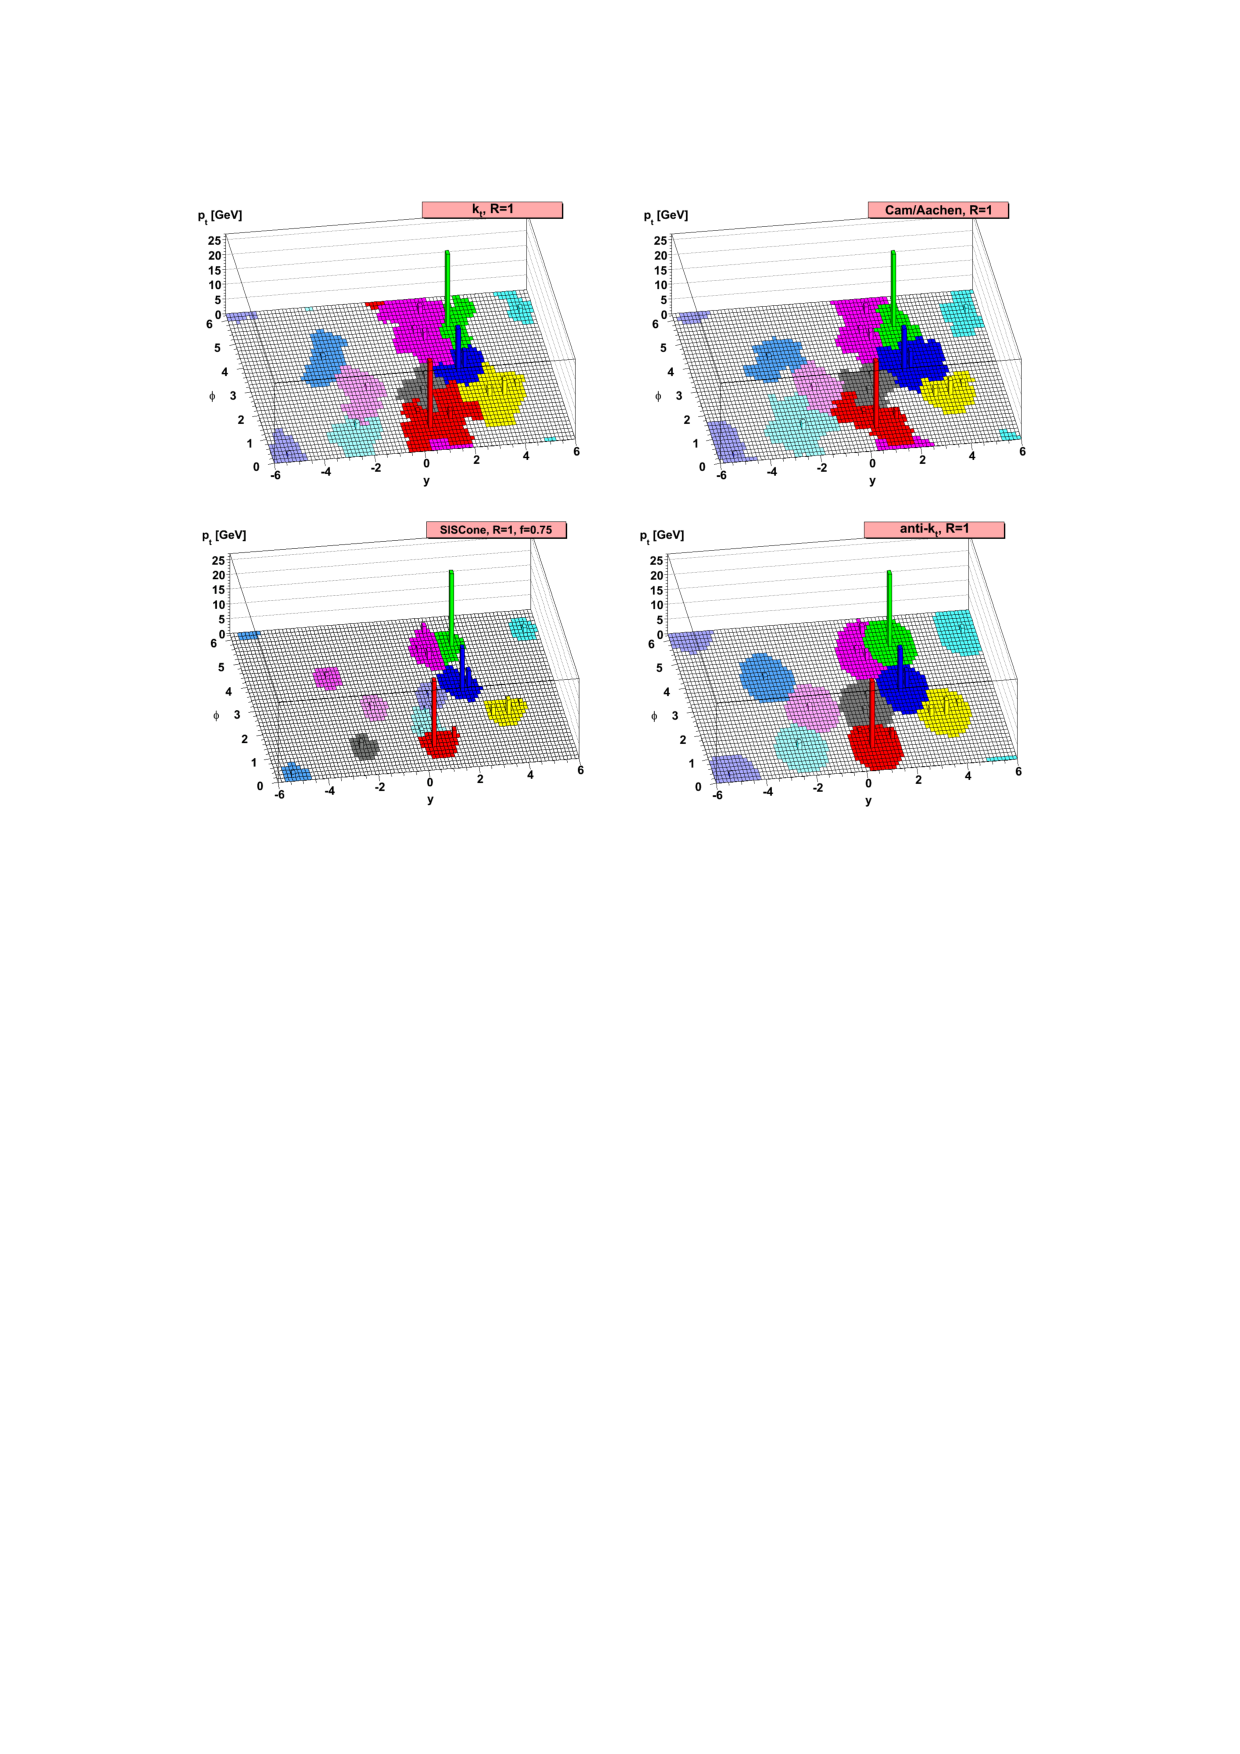
\includegraphics[width=0.8\textwidth]{figure/reco_antikt.pdf}
    \caption[Comparison of the jet clustering algorithm.]
    {
        Comparison of the jet clustering algorithm with randomly injected ghost particles, all using a radius parameter of $R=1$.
        The cluster boundaries in anti-\kt algorithm more determined by the hard center of the jets.
    }
    \label{fig:reco_antikt.png}
\end{figure}

\subsection{Jet corrections}
The kinematics of underlying partons from the strong interaction in the hard processes should be reflected to the jets.
This can be achieved by applying calibration factors obtained from detector responses and simulation assisted corrections to the jet kinematics (raw sum of all constituent particles).

The contribution from the pileup effect, leading to incorrect energy reconstruction of jets with charged particles candidates from pileup vertices, should be removed.
This process is called the charged hadron subtraction (CHS)~\cite{CMS:2020ebo}.

The contribution of neutral particles from pileup interactions, which can be estimated from the averaged energy area density $\rho_E$ for the event and the jet area, should also be removed.
This process is called the L1 pileup correction.

Further corrections such as L2L3 truth corrections should also be considered.
Those corrections are computed by directly comparing the true clustering momentum obtained from the constituent particles in simulation with the reconstruction momentum from the clustering algorithm.

The truth corrections can be further developed as the L2L3 residual corrections which are typically small.
To account for the differences in different detector responses in data and simulation, well-known jet emitting processes, such as the QCD multi-jet events can be studied.

\subsection{Jet identification}
Jet identification schemes are designed to reject noise such as jets forming around a lepton with soft radiation particle under the jet clustering algorithm.
It requires the reconstructed jet should be from good composition of various particle flavors (Fig.~\ref{fig:reco_jet}) to help identify jets originating from QCD particles.
\begin{figure}\centering
    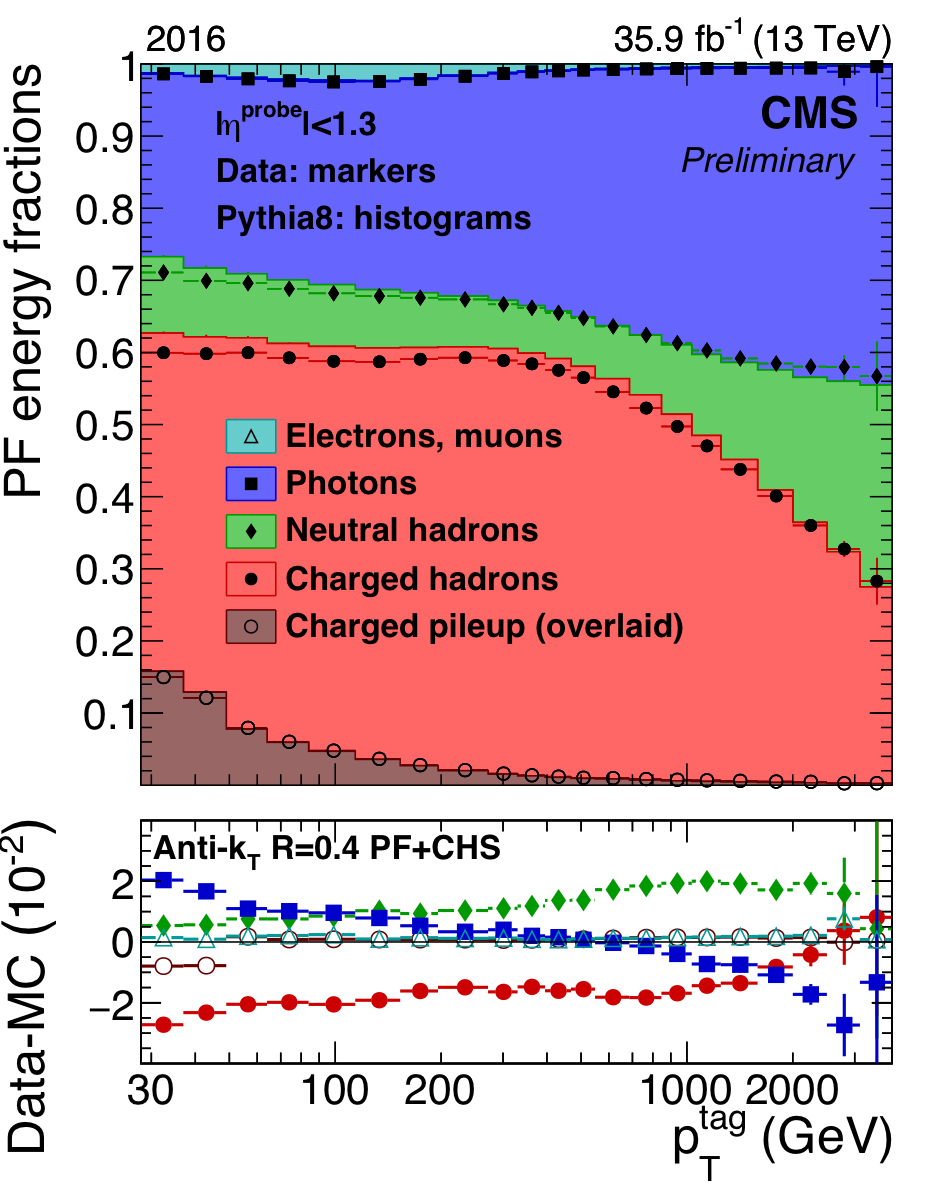
\includegraphics[width=0.4\textwidth]{figure/reco_jet16.png}
    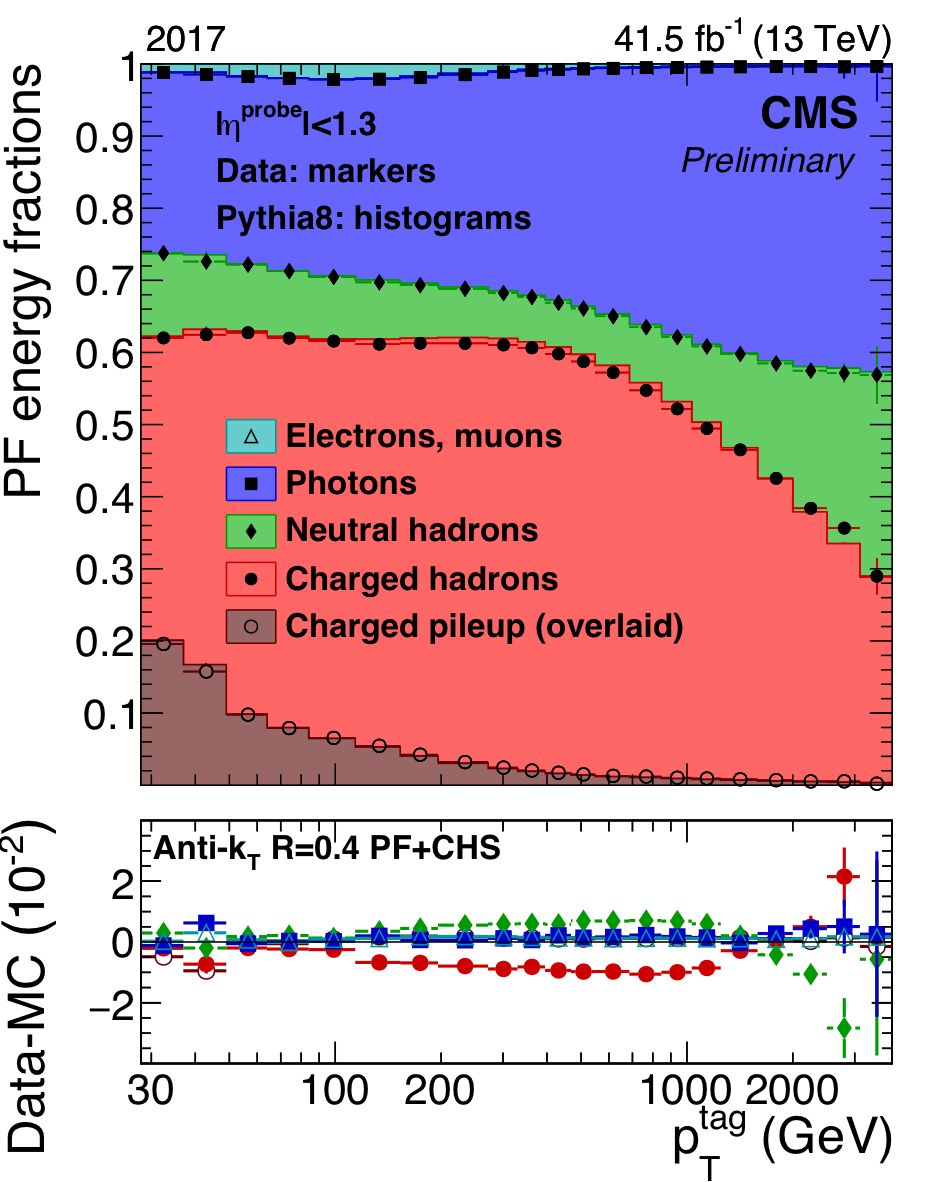
\includegraphics[width=0.4\textwidth]{figure/reco_jet17.png}
    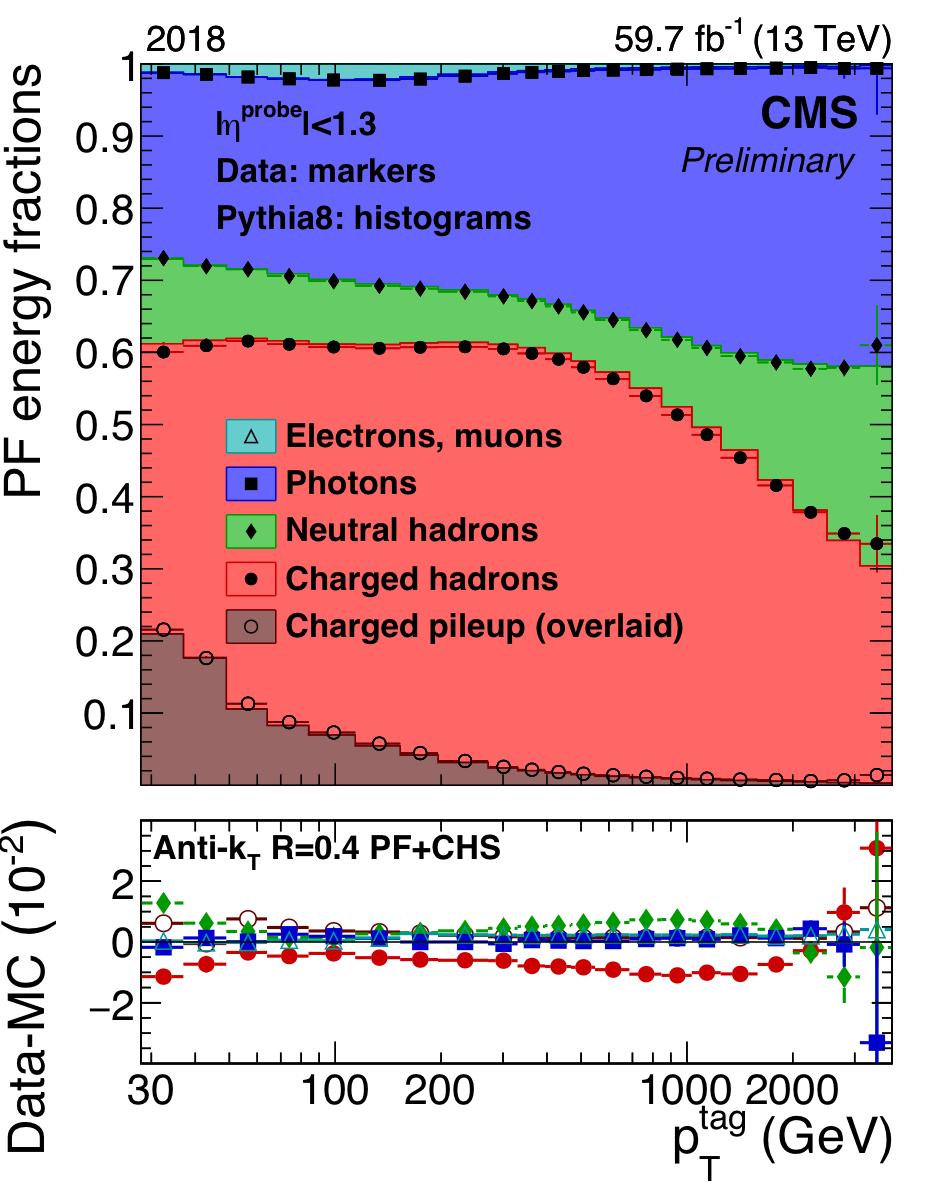
\includegraphics[width=0.4\textwidth]{figure/reco_jet18.png}
    \caption[Jet energy composition of various particle-flow candidates.]
    {
        Jet energy composition of various particle-flow candidates.
        Jets are clustered using the anti-\kt algorithm with size parameter $R=0.4$ during RunII.
    }
    \label{fig:reco_jet}
\end{figure}

The cuts used for jet identification at a loose working point for 2016 samples and a tight working point for 2017 and 2018 samples, both at around $99\%$ efficiency of selecting genuine jets.
All the jets are required to be within $|\eta|<2.4$ region and the detailed cut value in this analysis can be found in Table~\ref{tab:reco_jetid}.
\begin{table}
    \caption{Criteria of jet identification at different working points.}
    \label{tab:reco_jetid}
    \centering
    \begin{tabular}{ccc}
        \hline
        Variable & Loose & Tight\\
        \hline
        Neutral hadron energy fraction $<$ & 0.99 & 0.90\\
        Neutral EM energy fraction $<$ & 0.99 & 0.90\\
        Number of constituents $>$ 1 & 1\\
        Charged hadron energy fraction $>$ & 0 & 0\\
        Charged EM energy fraction $<$ & 0.99 & -\\ 
        Charged multiplicity $>$ & 0 & 0\\
        \hline
    \end{tabular}
\end{table}

\subsection{Jet flavor tagging}
The underlying parton flavor could be inferred from the constituents of the jets, however, not 100$\%$ correct in data.
Jets passing some threshold of the discriminator are typically called flavor tagged jets.

Jets with the underlying \PQb quark have relatively longer lifetime ($\mathcal{O}(\ten{-12})$ s) since the \PQb quark decays are suppressed by the elements $V_{\PQu\PQb}$ and $V_{\PQc\PQb}$ in the CKM matrix.
These b hadrons can propagate a longer distance from a few mm to one cm, and thus jets originating from \PQb quarks have signatures that is more easily identified.
The flight distance can be calculated with a \PQb hadron with mass $m$ on the order of $\approx 5\GeV$, energy $E$ on the order of $\approx 50 \GeV$, and an average lifetime $\tau$ on the order of $\approx \ten{-12}$ sec as 
\begin{linenomath}\begin{equation}\begin{aligned}\label{eq:reco_bjet}
    d_{\mathrm{flight}} &\approx v\tau\sqrt{1+(\frac{p}{mc})^2} \approx c\tau\frac{E}{mc^2} \\
                        &\approx 10^{-2} \mathrm{m}
\end{aligned}\end{equation}\end{linenomath}
This displacement creates a secondary vertex (SV) with significant transverse distance from the primary vertex illustrated in Fig.~\ref{fig:reco_bjet}.
\begin{figure}\centering
    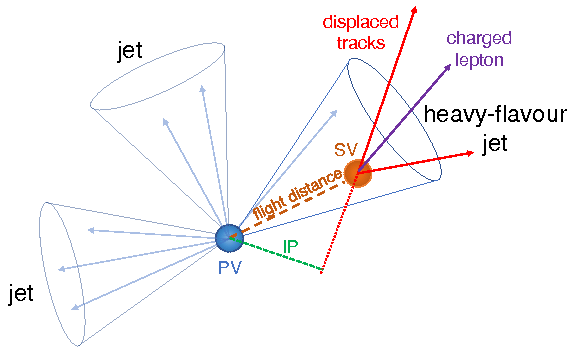
\includegraphics[width=0.7\textwidth]{figure/reco_bjet.png}
    \caption[Illustration of variable useful for \PQb tagging algorithm.]
    {
        Illustration of a heavy-flavour jet with a secondary vertex (SV) from the decay of a \PQb or \PQc hadron resulting in charged-particle tracks (including possibly a soft lepton) that are displaced with respect to the primary interaction vertex (PV), and hence with a large impact parameter (IP) value. 
    }
    \label{fig:reco_bjet}
\end{figure}

The features above can be used to compute a ML-based combined secondary vertex (CSV) discriminating factor~\cite{CMS:bjet_eff}.
It has been widely used in the CMS experiment for the \PQb jet identification during RunI, and has been improved with a deep neural network (DNN) during RunII to cope with higher pilup environment.
The improved CSV  discriminator, called \DeepCSV, uses information such as the impact parameters with respect to the primary vertices and the mass of the secondary vertex.
The \PQb tagging efficiency and misidentified efficiency under \DeepCSV discriminator are shown in Fig.~\ref{fig:reco_beff} and Fig.~\ref{fig:reco_misb}, respectively.

\begin{figure}\centering
    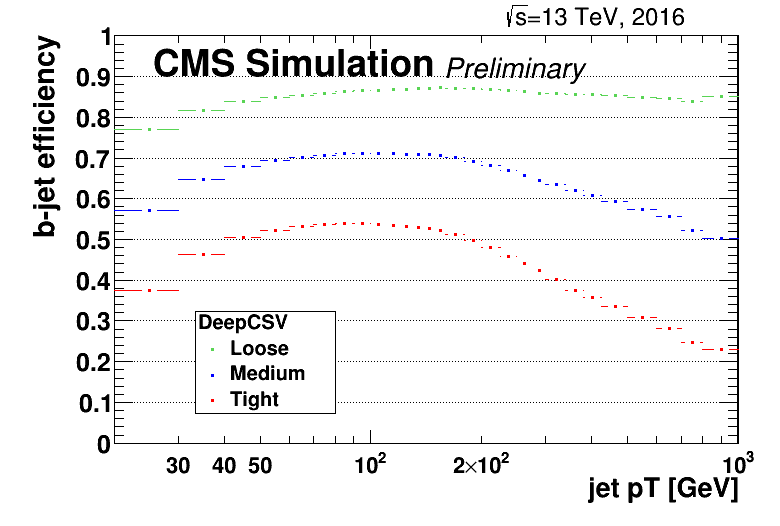
\includegraphics[width=0.7\textwidth]{figure/reco_beff.png}
    \caption
    {
        The efficiency of \PQb tagging as a function of the jet transverse momentum for the \DeepCSV algorithms. 
    }
    \label{fig:reco_beff}
\end{figure}

\begin{figure}\centering
    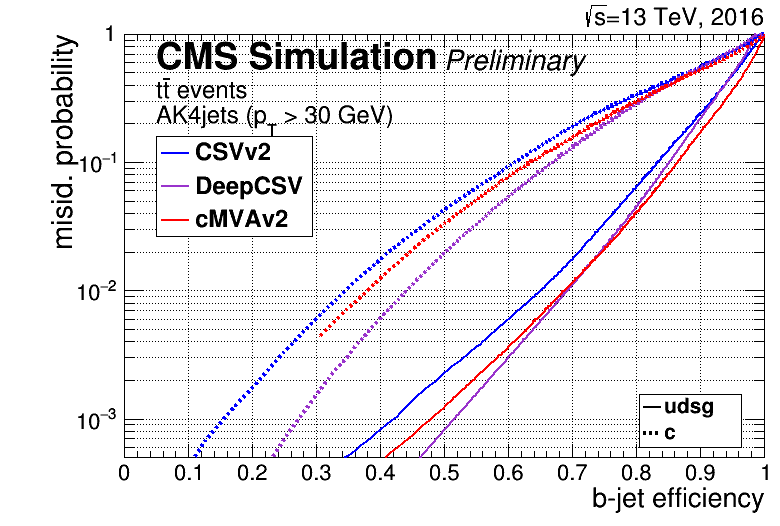
\includegraphics[width=0.7\textwidth]{figure/reco_misb.png}
    \caption[\PQb misidentified efficiency as a function of the \PQb tagging efficiency.]
    {
        Performance of the \PQb jet identification efficiency algorithms demonstrating the probability for non-b jets to be misidentified as \PQb jet as a function of the efficiency to correctly identify \PQb jets. 
        The curves are obtained on simulated \ttbar events using jets within tracker acceptance with $\PT>30 \GeV$, \PQb jets from gluon splitting to a pair of \PQb quarks are considered as \PQb jets.
    }
    \label{fig:reco_misb}
\end{figure}
